%!TEX root = 3_FormalAbstraction inLTLUnderUncertainty.tex

Motivated by space exploration applications we consider an autonomous rover tasked with identifying and collecting scientific samples.


\textbf{Rover model.} Without loss of generality, we consider a simple rover model as a point mass affected by stochastic disturbances on the state transitions. We assume that the position of the rover cannot be measured exactly. 
We model its dynamics as
\begin{align}
	x_{k+1}&=\begin{bmatrix}
		1&0\\
		0&1
	\end{bmatrix} x_{k} + \begin{bmatrix}
		1&0\\
		0&1
	\end{bmatrix} u_k+ w_k\\
z_k&=\begin{bmatrix}
		1&0\\
		0&1
	\end{bmatrix}x_k+v_k
\end{align}
with $w_k\sim \CA N \left(0,\begin{bmatrix}.4&-.2\\-.2&.4\end{bmatrix}\right)$ and $v_k\sim \CA N \left(0,\begin{bmatrix}1&.1\\.1&1\end{bmatrix}\right)$

A finite abstraction $M_{syst}$ of this model is constructed as outlined in the previous section by discretizing the input space $[-1,1]^2$ with nine discrete inputs, and the state space $[-10, 10]^2$ with grid points separated by $(0.76481, 0.64426)$.

\begin{figure}
	% This file was created by matplotlib2tikz v0.6.14.
\centering
\begin{tikzpicture}
\newlength\figurewidth
\newlength\figureheight
\setlength\figurewidth{\columnwidth}
\setlength\figureheight{.4\columnwidth}
\definecolor{color0}{rgb}{0.12156862745098,0.466666666666667,0.705882352941177}

\begin{axis}[scale =.8,
xlabel={$\delta$},
ylabel={$\epsilon$},
xmin=-0.01395, xmax=0.25,
ymin=0.8, ymax=1.45222764450879,
width=\figurewidth,
height=\figureheight,
% tick align=outside,
% tick pos=left,
x grid style={lightgray!92.026143790849673!black},
y grid style={lightgray!92.026143790849673!black},
axis y line=left,
axis x line=middle,
every axis x label/.style={
    at={(ticklabel* cs:1.05)}
}
]
\addplot [semithick, color0, forget plot,  mark=*,mark options={scale=.84}]
table {%
0.001 1.4272384844875
0.0167368421052632 1.22339465219428
0.0324736842105263 1.16617411196529
0.0482105263157895 1.13191279574885
0.0639473684210526 1.10601589042324
0.0796842105263158 1.08400668945514
0.0954210526315789 1.06721503359466
0.111157894736842 1.05265893349788
0.126894736842105 1.04157018327801
0.142631578947368 1.02417176675944
0.158368421052632 1.01254639660019
0.174105263157895 1.00120158889137
0.189842105263158 0.991557539021032
0.205578947368421 0.982277989301703
0.221315789473684 0.97353496742902
0.237052631578947 0.965239656823681
0.252789473684211 0.960158902624749
0.268526315789474 0.951512372393061
0.284263157894737 0.927455284061691
0.3 0.935781247731614
};
\end{axis}

\end{tikzpicture}
	\caption{Trade-off between $\epsilon$ and $\delta$.  }
\end{figure}

\textbf{Environment model.} We consider exploration in a partially unknown environment. In particular, there are two potential target regions $T_1$ and $T_2$ where the probability of encountering a sample has been assessed as 0.5 and 0.6, respectively. In addition, there are two potential obstacle regions $O_1$ and $O_2$ where estimates based on satellite imagery give probabilities 0.1 and 0.3 that the rover can not traverse the obstacle safely. For both target and obstacle regions, we assume that the true nature of the region can be measured when the rover is within a certain distance of the regions. The regions are illustrated in Figs. \ref{fig:exp1} and \ref{fig:exp2}.

This environment model can be modeled as a finite-state MDP $M_{env}$. Furthermore, we model a failure probability of 0.01 at each step with an additional MDP $M_{fail}$.

\textbf{Specification.} The objective is to collect a sample while avoiding unsafe regions. To this end, we consider the specification
\begin{equation}
	\varphi = \lozenge \texttt{sample} \land \left( \lnot \texttt{fail} \; \mathcal {U} \; \texttt{sample} \right),
\end{equation}
where the atomic proposition \texttt{sample} is true if the rover is in a target region that contains a sample, and the atomic proposition \texttt{fail} is defined as being in an obstacle region that contains an obstacle, or that the system is in failure mode.

\textbf{Results.} We consider the aggregate system $M_{syst} \times M_{env} \times M_{fail}$ which is an MDP with 9 inputs and 277182 states. The specification $\varphi$ can be converted into a deterministic finite automaton. Via \eqref{eq:prob:robust_optimal} we can synthesize a control policy. Figs. \ref{fig:exp1} and \ref{fig:exp2} depict trajectories generated by the control policies, and the estimated probability that the specification can be satisfied, under two different resolutions of the unknown environment. In both experiments only $T_2$ contains a sample, and $O_1$ contains an obstacle. The difference is that in Fig. \ref{fig:exp1} also $O_2$ contains an obstacle but in Fig. \ref{fig:exp2} this region can be safely transversed.

\begin{figure}
	\footnotesize
	\setlength\figurewidth{\columnwidth} 
	\setlength\figureheight{0.6\columnwidth} 

	% This file was created by matplotlib2tikz v0.6.14.
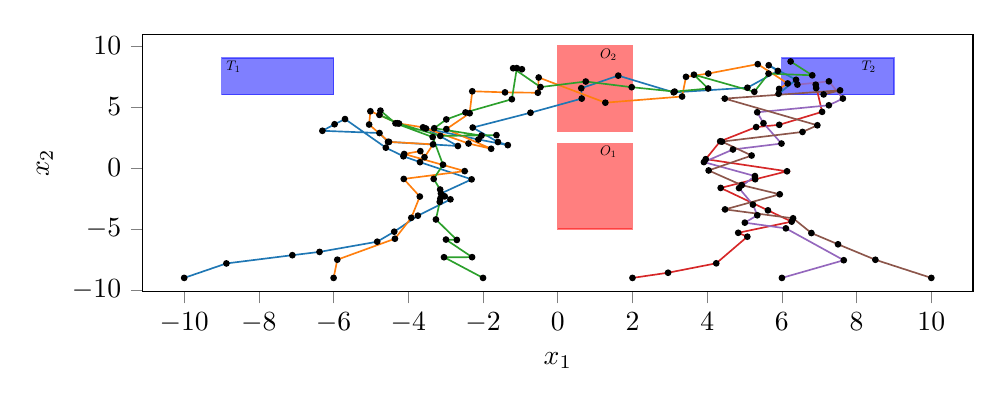
\begin{tikzpicture}

\definecolor{color1}{rgb}{1,0.498039215686275,0.0549019607843137}
\definecolor{color0}{rgb}{0.12156862745098,0.466666666666667,0.705882352941177}
\definecolor{color3}{rgb}{0.83921568627451,0.152941176470588,0.156862745098039}
\definecolor{color2}{rgb}{0.172549019607843,0.627450980392157,0.172549019607843}
\definecolor{color5}{rgb}{0.549019607843137,0.337254901960784,0.294117647058824}
\definecolor{color4}{rgb}{0.580392156862745,0.403921568627451,0.741176470588235}

\begin{axis}[
xlabel={$x_1$},
ylabel={$x_2$},
xmin=-11.1088588047251, xmax=11.1145664581499,
ymin=-10.1108621762447, ymax=10.9576601036307,
width=\figurewidth,
height=\figureheight,
tick align=outside,
tick pos=left,
mark size=1,
x grid style={lightgray!92.026143790849673!black},
y grid style={lightgray!92.026143790849673!black}
]
\addplot [only marks, draw=black, fill=black, colormap/viridis]
table{%
x                      y
-1.000000000000000e+01 -9.000000000000000e+00
-8.869595294321220e+00 -7.814207719224903e+00
-7.104778400743559e+00 -7.140354399223419e+00
-6.376752541526766e+00 -6.870554896721502e+00
-4.832702844468539e+00 -6.036032413666041e+00
-4.377547654253716e+00 -5.216915548266608e+00
-3.744230908366174e+00 -3.905880113729608e+00
-2.871984978581734e+00 -2.567990703687725e+00
-3.127375571989979e+00 -2.090610019084363e+00
-2.305771899885637e+00 -9.338180566109633e-01
-3.687373068419801e+00 +4.769618066414293e-01
-4.131753222593663e+00 +9.557682476343059e-01
-4.601633165510158e+00 +1.661042239367786e+00
-5.694730614871723e+00 +4.003513878529873e+00
-5.973575212285128e+00 +3.578554273124150e+00
-6.299886148045688e+00 +3.044114991420233e+00
-4.771656903671562e+00 +2.858962077904698e+00
-4.543639365229525e+00 +2.139567825321754e+00
-2.673138926724003e+00 +1.798961623791945e+00
-3.527414786094551e+00 +3.231833707854521e+00
-2.124252800165384e+00 +2.332430078604584e+00
-1.336517727306551e+00 +1.867196593378676e+00
-1.601443252054275e+00 +2.126202270702624e+00
-2.276211315148957e+00 +3.308254449757351e+00
-7.301645225187249e-01 +4.522420844572547e+00
+6.421309072702257e-01 +5.679192620151055e+00
+6.291550303486995e-01 +6.527896371328548e+00
+1.619950872445812e+00 +7.559823424104585e+00
+3.103218944956174e+00 +6.190024650395538e+00
+5.076329139729479e+00 +6.568676876712611e+00
+5.892120984615905e+00 +7.942903477538653e+00
+5.647060738990990e+00 +8.410805253485940e+00
+6.378542919870930e+00 +7.216198212323969e+00
+5.911651447016797e+00 +6.074808626739333e+00
};
\addplot [only marks, draw=black, fill=black, colormap/viridis]
table{%
x                      y
-6.000000000000000e+00 -9.000000000000000e+00
-5.901406929599968e+00 -7.508199438071110e+00
-4.358884763233826e+00 -5.792082591551480e+00
-3.919800671528496e+00 -4.077694923566842e+00
-3.692867013779527e+00 -2.339134536400095e+00
-4.122397810293728e+00 -8.975301878708711e-01
-2.490405176513862e+00 -2.573953379208296e-01
-4.111781121286302e+00 +1.145086563115543e+00
-3.677892980298973e+00 +1.377137896197289e+00
-3.566602837148350e+00 +8.815148406364688e-01
-3.338101562637621e+00 +1.932094838504950e+00
-4.516623627187172e+00 +2.134782889471700e+00
-5.049009747014780e+00 +3.556356142323278e+00
-5.015975542724512e+00 +4.642632272866249e+00
-4.249031141395299e+00 +3.638868112650753e+00
-3.606475659338956e+00 +3.327243509372837e+00
-2.389126541991601e+00 +2.001450651124150e+00
-1.783057348634495e+00 +1.573015875488078e+00
-2.981625704030834e+00 +3.183156711833124e+00
-2.358357517805116e+00 +4.479839517723944e+00
-2.288659157327666e+00 +6.279107959374064e+00
-1.411436975902111e+00 +6.189266978612975e+00
-5.320073996643725e-01 +6.157716555765220e+00
-5.104133024329928e-01 +7.405451568002405e+00
+1.274177610274697e+00 +5.346446814476317e+00
+3.328125868896929e+00 +5.848995543358567e+00
+3.432597856511344e+00 +7.459258972502006e+00
+4.030094855910188e+00 +7.728847292266309e+00
+5.354424702892910e+00 +8.500182463536220e+00
+6.155873129399546e+00 +6.918829831869020e+00
+5.925808542673061e+00 +6.475595415762200e+00
};
\addplot [only marks, draw=black, fill=black, colormap/viridis]
table{%
x                      y
-2.000000000000000e+00 -9.000000000000000e+00
-3.044462714452268e+00 -7.306350162100894e+00
-2.293090798054657e+00 -7.301138964922043e+00
-2.992445270727864e+00 -5.860237642906498e+00
-2.700570628355699e+00 -5.891003937213707e+00
-3.261421640643176e+00 -4.215783895557847e+00
-3.158411977295807e+00 -2.780961678014854e+00
-3.143450533987836e+00 -2.507508068387384e+00
-3.025567040118594e+00 -2.323985887674691e+00
-3.147878570292180e+00 -1.765176888234320e+00
-3.321097798094850e+00 -8.960733607114131e-01
-3.071809481398453e+00 +2.656018153234110e-01
-3.347289674472285e+00 +2.525143550310250e+00
-4.343077763169791e+00 +3.655246402097009e+00
-4.746507006214285e+00 +4.694914521302897e+00
-4.773216787388434e+00 +4.346197557892083e+00
-4.295952786822955e+00 +3.660497376626418e+00
-3.143953286965482e+00 +2.625049791199087e+00
-1.641162836868084e+00 +2.688373056222609e+00
-2.041754565063155e+00 +2.649157162515526e+00
-3.306752490703531e+00 +3.253350556635815e+00
-2.983336851770111e+00 +3.971825313172622e+00
-2.469010596282821e+00 +4.546595568617136e+00
-1.228788797359903e+00 +5.627707538998200e+00
-1.094952620493618e+00 +8.175427155795038e+00
-9.592574172669480e-01 +8.082721342294306e+00
-1.194386354456936e+00 +8.165264896530068e+00
-4.616822792871155e-01 +6.621700444105216e+00
+7.497631277014686e-01 +7.076610441120152e+00
+1.979746828542337e+00 +6.612237335050672e+00
+3.128826364302311e+00 +6.253528797214032e+00
+4.025272616622998e+00 +6.503242452969750e+00
+3.645362150228443e+00 +7.636106778389254e+00
+5.261846571766094e+00 +6.237023538647955e+00
+5.641826018152110e+00 +7.725113353647728e+00
+6.812612257678752e+00 +7.585618827435113e+00
+6.232989074320007e+00 +8.719742643797003e+00
};
\addplot [only marks, draw=black, fill=black, colormap/viridis]
table{%
x                      y
+2.000000000000000e+00 -9.000000000000000e+00
+2.952866870372958e+00 -8.576100227432466e+00
+4.242197553383458e+00 -7.804545716747594e+00
+5.074855341092752e+00 -5.625352120055734e+00
+4.830608053317017e+00 -5.307135825638624e+00
+6.260668707794887e+00 -4.393024727214535e+00
+5.626132234535231e+00 -3.468882934108938e+00
+4.360920432033688e+00 -1.633814410374898e+00
+5.283892683157318e+00 -9.239872896419613e-01
+6.137055506057617e+00 -2.713402990434055e-01
+3.960819582615776e+00 +7.198393840378496e-01
+4.348495153676051e+00 +2.182925104805387e+00
+5.310490549051644e+00 +3.346073054040058e+00
+5.927805236978374e+00 +3.532146335797724e+00
+7.076206486765265e+00 +4.595056538443954e+00
+6.905541839334503e+00 +6.818868569963236e+00
+6.916859672204205e+00 +6.538704789396275e+00
};
\addplot [only marks, draw=black, fill=black, colormap/viridis]
table{%
x                      y
+6.000000000000000e+00 -9.000000000000000e+00
+7.656026307682226e+00 -7.552110273740422e+00
+6.106733751763857e+00 -4.944778792524008e+00
+5.007607308637190e+00 -4.476890270578113e+00
+5.340307715623565e+00 -3.870524755975019e+00
+5.223674090042989e+00 -2.999138613814250e+00
+4.852825372926093e+00 -1.649771429171313e+00
+5.277460910519775e+00 -6.637444320456167e-01
+3.912214555867033e+00 +4.809921810937652e-01
+4.689101241974543e+00 +1.514074549520304e+00
+5.988818016236550e+00 +1.998528533661037e+00
+5.506348480377154e+00 +3.663415125077347e+00
+5.339192804183695e+00 +4.558762439747721e+00
+7.256112587009863e+00 +5.131362769874022e+00
+7.631959808780144e+00 +5.683576842740282e+00
+7.257947121647226e+00 +7.090711607035485e+00
+6.414874444391497e+00 +6.824546651611620e+00
};
\addplot [only marks, draw=black, fill=black, colormap/viridis]
table{%
x                      y
+1.000000000000000e+01 -9.000000000000000e+00
+8.501744459872617e+00 -7.514163496353530e+00
+7.502543301317530e+00 -6.247529485824156e+00
+6.789481505237688e+00 -5.327060783448672e+00
+6.299648866376312e+00 -4.120122662433571e+00
+4.477615169608585e+00 -3.392450768338643e+00
+5.941939396771113e+00 -2.155271399521218e+00
+4.924919113275441e+00 -1.405474597240854e+00
+4.038299633666932e+00 -2.035680327253797e-01
+5.189304536388701e+00 +1.018679026545901e+00
+4.395910542655945e+00 +2.158524989021073e+00
+6.551109435674287e+00 +2.948566939226978e+00
+6.949044679173154e+00 +3.493783802114474e+00
+4.470283883624948e+00 +5.678295462897534e+00
+7.557669000755279e+00 +6.353439694488499e+00
+7.116516078033896e+00 +6.021511860498869e+00
};
\path [draw=red, fill=red, opacity=0.5] (axis cs:2,-5)
--(axis cs:2,2)
--(axis cs:0,2)
--(axis cs:0,-5)
--cycle;

\path [draw=red, fill=red, opacity=0.5] (axis cs:2,3)
--(axis cs:2,10)
--(axis cs:0,10)
--(axis cs:0,3)
--cycle;

\path [draw=blue, fill=blue, opacity=0.5] (axis cs:-6,6)
--(axis cs:-6,9)
--(axis cs:-9,9)
--(axis cs:-9,6)
--cycle;

\path [draw=blue, fill=blue, opacity=0.5] (axis cs:9,6)
--(axis cs:9,9)
--(axis cs:6,9)
--(axis cs:6,6)
--cycle;

\addplot [semithick, color0, forget plot]
table {%
-10 -9
-8.86959529432122 -7.8142077192249
-7.10477840074356 -7.14035439922342
-6.37675254152677 -6.8705548967215
-4.83270284446854 -6.03603241366604
-4.37754765425372 -5.21691554826661
-3.74423090836617 -3.90588011372961
-2.87198497858173 -2.56799070368773
-3.12737557198998 -2.09061001908436
-2.30577189988564 -0.933818056610963
-3.6873730684198 0.476961806641429
-4.13175322259366 0.955768247634306
-4.60163316551016 1.66104223936779
-5.69473061487172 4.00351387852987
-5.97357521228513 3.57855427312415
-6.29988614804569 3.04411499142023
-4.77165690367156 2.8589620779047
-4.54363936522953 2.13956782532175
-2.673138926724 1.79896162379194
-3.52741478609455 3.23183370785452
-2.12425280016538 2.33243007860458
-1.33651772730655 1.86719659337868
-1.60144325205428 2.12620227070262
-2.27621131514896 3.30825444975735
-0.730164522518725 4.52242084457255
0.642130907270226 5.67919262015106
0.629155030348699 6.52789637132855
1.61995087244581 7.55982342410458
3.10321894495617 6.19002465039554
5.07632913972948 6.56867687671261
5.8921209846159 7.94290347753865
5.64706073899099 8.41080525348594
6.37854291987093 7.21619821232397
5.9116514470168 6.07480862673933
};
\addplot [semithick, color1, forget plot]
table {%
-6 -9
-5.90140692959997 -7.50819943807111
-4.35888476323383 -5.79208259155148
-3.9198006715285 -4.07769492356684
-3.69286701377953 -2.3391345364001
-4.12239781029373 -0.897530187870871
-2.49040517651386 -0.25739533792083
-4.1117811212863 1.14508656311554
-3.67789298029897 1.37713789619729
-3.56660283714835 0.881514840636469
-3.33810156263762 1.93209483850495
-4.51662362718717 2.1347828894717
-5.04900974701478 3.55635614232328
-5.01597554272451 4.64263227286625
-4.2490311413953 3.63886811265075
-3.60647565933896 3.32724350937284
-2.3891265419916 2.00145065112415
-1.7830573486345 1.57301587548808
-2.98162570403083 3.18315671183312
-2.35835751780512 4.47983951772394
-2.28865915732767 6.27910795937406
-1.41143697590211 6.18926697861298
-0.532007399664372 6.15771655576522
-0.510413302432993 7.40545156800241
1.2741776102747 5.34644681447632
3.32812586889693 5.84899554335857
3.43259785651134 7.45925897250201
4.03009485591019 7.72884729226631
5.35442470289291 8.50018246353622
6.15587312939955 6.91882983186902
5.92580854267306 6.4755954157622
};
\addplot [semithick, color2, forget plot]
table {%
-2 -9
-3.04446271445227 -7.30635016210089
-2.29309079805466 -7.30113896492204
-2.99244527072786 -5.8602376429065
-2.7005706283557 -5.89100393721371
-3.26142164064318 -4.21578389555785
-3.15841197729581 -2.78096167801485
-3.14345053398784 -2.50750806838738
-3.02556704011859 -2.32398588767469
-3.14787857029218 -1.76517688823432
-3.32109779809485 -0.896073360711413
-3.07180948139845 0.265601815323411
-3.34728967447229 2.52514355031025
-4.34307776316979 3.65524640209701
-4.74650700621429 4.6949145213029
-4.77321678738843 4.34619755789208
-4.29595278682296 3.66049737662642
-3.14395328696548 2.62504979119909
-1.64116283686808 2.68837305622261
-2.04175456506316 2.64915716251553
-3.30675249070353 3.25335055663581
-2.98333685177011 3.97182531317262
-2.46901059628282 4.54659556861714
-1.2287887973599 5.6277075389982
-1.09495262049362 8.17542715579504
-0.959257417266948 8.08272134229431
-1.19438635445694 8.16526489653007
-0.461682279287116 6.62170044410522
0.749763127701469 7.07661044112015
1.97974682854234 6.61223733505067
3.12882636430231 6.25352879721403
4.025272616623 6.50324245296975
3.64536215022844 7.63610677838925
5.26184657176609 6.23702353864796
5.64182601815211 7.72511335364773
6.81261225767875 7.58561882743511
6.23298907432001 8.719742643797
};
\addplot [semithick, color3, forget plot]
table {%
2 -9
2.95286687037296 -8.57610022743247
4.24219755338346 -7.80454571674759
5.07485534109275 -5.62535212005573
4.83060805331702 -5.30713582563862
6.26066870779489 -4.39302472721454
5.62613223453523 -3.46888293410894
4.36092043203369 -1.6338144103749
5.28389268315732 -0.923987289641961
6.13705550605762 -0.271340299043406
3.96081958261578 0.71983938403785
4.34849515367605 2.18292510480539
5.31049054905164 3.34607305404006
5.92780523697837 3.53214633579772
7.07620648676526 4.59505653844395
6.9055418393345 6.81886856996324
6.9168596722042 6.53870478939627
};
\addplot [semithick, color4, forget plot]
table {%
6 -9
7.65602630768223 -7.55211027374042
6.10673375176386 -4.94477879252401
5.00760730863719 -4.47689027057811
5.34030771562356 -3.87052475597502
5.22367409004299 -2.99913861381425
4.85282537292609 -1.64977142917131
5.27746091051977 -0.663744432045617
3.91221455586703 0.480992181093765
4.68910124197454 1.5140745495203
5.98881801623655 1.99852853366104
5.50634848037715 3.66341512507735
5.3391928041837 4.55876243974772
7.25611258700986 5.13136276987402
7.63195980878014 5.68357684274028
7.25794712164723 7.09071160703548
6.4148744443915 6.82454665161162
};
\addplot [semithick, color5, forget plot]
table {%
10 -9
8.50174445987262 -7.51416349635353
7.50254330131753 -6.24752948582416
6.78948150523769 -5.32706078344867
6.29964886637631 -4.12012266243357
4.47761516960859 -3.39245076833864
5.94193939677111 -2.15527139952122
4.92491911327544 -1.40547459724085
4.03829963366693 -0.20356803272538
5.1893045363887 1.0186790265459
4.39591054265594 2.15852498902107
6.55110943567429 2.94856693922698
6.94904467917315 3.49378380211447
4.47028388362495 5.67829546289753
7.55766900075528 6.3534396944885
7.1165160780339 6.02151186049887
};
\node at (axis cs:1,1)[
  scale=0.5,
  anchor=base west,
  text=black,
  rotate=0.0
]{ $O_1$};
\node at (axis cs:1,9)[
  scale=0.5,
  anchor=base west,
  text=black,
  rotate=0.0
]{ $O_2$};
\node at (axis cs:-9,8)[
  scale=0.5,
  anchor=base west,
  text=black,
  rotate=0.0
]{ $T_1$};
\node at (axis cs:8,8)[
  scale=0.5,
  anchor=base west,
  text=black,
  rotate=0.0
]{ $T_2$};
\end{axis}

\end{tikzpicture}
	\setlength\figureheight{0.4\columnwidth} 

	% This file was created by matplotlib2tikz v0.6.14.
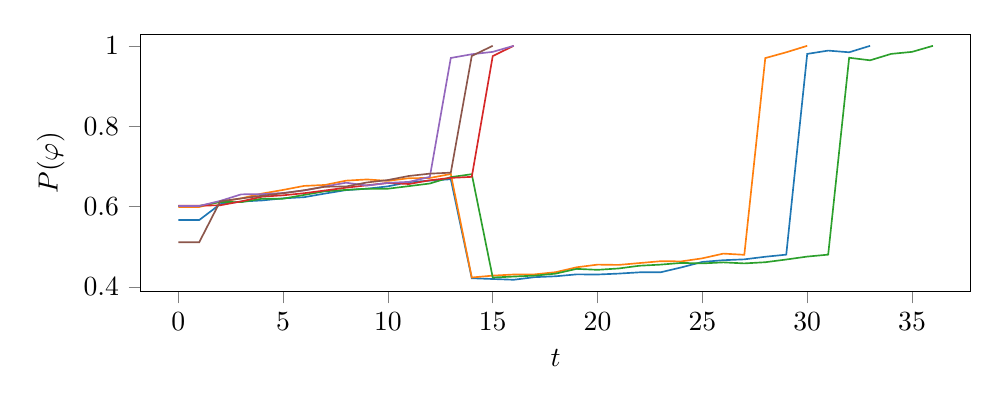
\begin{tikzpicture}

\definecolor{color1}{rgb}{1,0.498039215686275,0.0549019607843137}
\definecolor{color0}{rgb}{0.12156862745098,0.466666666666667,0.705882352941177}
\definecolor{color3}{rgb}{0.83921568627451,0.152941176470588,0.156862745098039}
\definecolor{color2}{rgb}{0.172549019607843,0.627450980392157,0.172549019607843}
\definecolor{color5}{rgb}{0.549019607843137,0.337254901960784,0.294117647058824}
\definecolor{color4}{rgb}{0.580392156862745,0.403921568627451,0.741176470588235}

\begin{axis}[
xlabel={$t$},
ylabel={$\mathbb{P}(\varphi)$},
xmin=-1.8, xmax=37.8,
ymin=0.38853456067633, ymax=1.02911740187259,
width=\figurewidth,
height=\figureheight,
tick align=outside,
tick pos=left,
x grid style={lightgray!92.026143790849673!black},
y grid style={lightgray!92.026143790849673!black}
]
\addplot [semithick, color0, forget plot]
table {%
0 0.566291945691099
1 0.566291945691099
2 0.605882976959095
3 0.612354132971019
4 0.615146535917152
5 0.620313388350838
6 0.623169341037894
7 0.632266923722546
8 0.640795190330476
9 0.64428856744584
10 0.650176429635556
11 0.660779548866506
12 0.664373678411201
13 0.667953572290617
14 0.421487160337076
15 0.419564608493884
16 0.417651962548887
17 0.424169566255033
18 0.426345484650421
19 0.431108756242508
20 0.430751120445197
21 0.433029533909929
22 0.436207218324974
23 0.436207218324974
24 0.448504360104309
25 0.462109503911388
26 0.466372172152465
27 0.468495540003818
28 0.474972821467856
29 0.480216364807438
30 0.979868029536619
31 0.988089397434187
32 0.983895865110246
33 1.00000000000003
};
\addplot [semithick, color1, forget plot]
table {%
0 0.598873106893363
1 0.598873106893363
2 0.611938797531012
3 0.620313388350838
4 0.632266923722546
5 0.641338529177884
6 0.651286575651904
7 0.653667661427169
8 0.664373678411201
9 0.667389245077004
10 0.663807726695736
11 0.670472509073791
12 0.671058796741362
13 0.680876876002895
14 0.423299602729996
15 0.428005120445258
16 0.430751120445197
17 0.431108756242508
18 0.436564779737749
19 0.448714044552832
20 0.455361601380584
21 0.454662990626655
22 0.459229983640598
23 0.463841336213989
24 0.463444874596063
25 0.471062027085172
26 0.482793941967823
27 0.479801326577619
28 0.969453775583137
29 0.983895865110246
30 1.00000000000003
};
\addplot [semithick, color2, forget plot]
table {%
0 0.601199049439663
1 0.601199049439663
2 0.611373258769312
3 0.610825977206025
4 0.61950569968835
5 0.61950569968835
6 0.628810791270583
7 0.637985226843664
8 0.641338529177884
9 0.64428856744584
10 0.64428856744584
11 0.65073129659484
12 0.657238925992285
13 0.673118973708607
14 0.680502261669169
15 0.423299602729996
16 0.425630605759241
17 0.428005120445258
18 0.432928711351226
19 0.444768945274215
20 0.442429168485533
21 0.445763301335716
22 0.452612154776499
23 0.455361601380584
24 0.459622816160484
25 0.458418097195606
26 0.460938662424354
27 0.458418097195606
28 0.461333021386082
29 0.468094526343635
30 0.475377924614331
31 0.480216364807438
32 0.970297252430312
33 0.963929119062114
34 0.979868029536619
35 0.984943443987629
36 1.00000000000003
};
\addplot [semithick, color3, forget plot]
table {%
0 0.60221316758681
1 0.60221316758681
2 0.603095656982768
3 0.612754055717539
4 0.624538495801648
5 0.62791668893401
6 0.633081343456916
7 0.639922816020793
8 0.646852485781285
9 0.652756759496805
10 0.658726606328146
11 0.655977449212481
12 0.665293062315518
13 0.671265524930602
14 0.673823637438148
15 0.974478764836217
16 1.00000000000003
};
\addplot [semithick, color4, forget plot]
table {%
0 0.601395515122941
1 0.601395515122941
2 0.61392554430982
3 0.630267741952442
4 0.630807082939585
5 0.633670305343681
6 0.639922816020793
7 0.649819559965179
8 0.659285200283324
9 0.652182261074434
10 0.658796362546444
11 0.661342844708322
12 0.673823637438148
13 0.969766480712513
14 0.979000636609888
15 0.984943431279268
16 1.00000000000003
};
\addplot [semithick, color5, forget plot]
table {%
0 0.511047337255817
1 0.511047337255817
2 0.612978700250407
3 0.620063167202848
4 0.626830204231395
5 0.633081343456916
6 0.640464676396021
7 0.649268206152165
8 0.649819559965179
9 0.659844019602223
10 0.665920200487818
11 0.67605034228333
12 0.681786379389656
13 0.684269702304902
14 0.974797775257462
15 1.00000000000003
};
\end{axis}

\end{tikzpicture}
	\caption{Above: six trajectories starting at different initial conditions. Below: estimated probability to satisfy the specification over time for the same trajectories. No sample is found in $T_1$, and $O_2$ can be safely transversed. Jumps occur in the probabilities when (non-)existence of samples are measured when the rover is close to the regions.}
	\label{fig:exp1}
\end{figure}

\begin{figure}
	\footnotesize
	\setlength\figurewidth{\columnwidth} 
	\setlength\figureheight{0.6\columnwidth} 

	% This file was created by matplotlib2tikz v0.6.14.
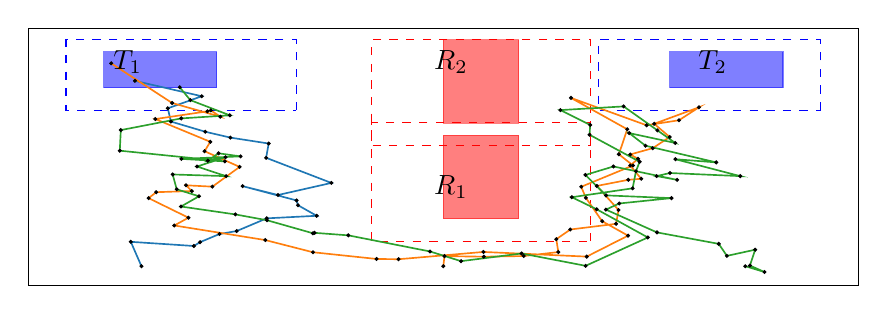
\begin{tikzpicture}

\definecolor{color1}{rgb}{1,0.498039215686275,0.0549019607843137}
\definecolor{color0}{rgb}{0.12156862745098,0.466666666666667,0.705882352941177}
\definecolor{color2}{rgb}{0.172549019607843,0.627450980392157,0.172549019607843}

\begin{axis}[
mark size = 0.5,
ticks=none,
xmin=-11, xmax=11,
ymin=-10.6290882408405, ymax=10.9823375352781,
width=\figurewidth,
height=\figureheight,
tick align=outside,
tick pos=left,
x grid style={lightgray!92.026143790849673!black},
y grid style={lightgray!92.026143790849673!black}
]
\addplot [only marks, draw=black, fill=black, colormap/viridis]
table{%
x                      y
-8.000000000000000e+00 -9.000000000000000e+00
-8.281791193811282e+00 -6.953277059756937e+00
-6.609947231673338e+00 -7.304755895777043e+00
-6.447420151999264e+00 -6.984253859219061e+00
-5.930025319876885e+00 -6.296279125763103e+00
-5.476123458484502e+00 -6.049868453584115e+00
-4.680375628377898e+00 -4.982516422756326e+00
-3.356608221836718e+00 -4.767445283086258e+00
-3.850337386959414e+00 -3.882953851781119e+00
-3.888519145722516e+00 -3.480146659512000e+00
-5.320305970691908e+00 -2.277119535242806e+00
-4.379722627893722e+00 -3.023297381626749e+00
-2.966831046751209e+00 -2.008805754832921e+00
-4.696058526749306e+00 +1.019091306738935e-01
-4.628219306657023e+00 +1.300100090541606e+00
-5.641564937919985e+00 +1.796635145522380e+00
-6.307184225641461e+00 +2.288130625455808e+00
-7.217828733789983e+00 +3.143921812081298e+00
-7.301911031188013e+00 +4.255956608402649e+00
-6.401344954223192e+00 +5.270680166902547e+00
-8.171856419882948e+00 +6.563080734161627e+00
};
\addplot [only marks, draw=black, fill=black, colormap/viridis]
table{%
x                      y
+0.000000000000000e+00 -9.000000000000000e+00
+2.985780663708160e-02 -8.155463278156050e+00
+1.071409254737555e+00 -8.202590105544974e+00
+2.130577217930679e+00 -8.147034783291767e+00
+3.046653997506764e+00 -7.814782310273142e+00
+2.993503950729483e+00 -6.732513426782055e+00
+3.364980364937721e+00 -5.919601911047740e+00
+4.577267269183741e+00 -5.442531058948178e+00
+4.641924364448064e+00 -4.277469389688367e+00
+4.066522550812240e+00 -2.261074508296681e+00
+4.900884132823337e+00 -1.747839224197387e+00
+5.242948546817824e+00 -1.658932790996334e+00
+4.951650027020797e+00 -5.458682191996835e-01
+5.160727075484108e+00 +1.786499818804027e-02
+4.951600531141041e+00 +3.796585040088380e-01
+5.548111410812709e+00 +9.093914656273301e-01
+5.998289710281483e+00 +1.845859092339620e+00
+5.586468819814069e+00 +2.958893844938457e+00
+6.773322394657046e+00 +4.341573264475908e+00
+6.244801362810740e+00 +3.255339248138667e+00
+5.386058184710604e+00 +2.832977405694789e+00
+3.382447161292124e+00 +5.131303079674516e+00
+4.874337596806267e+00 +2.495954941054408e+00
+4.650503806334480e+00 +3.995285095184848e-01
+5.025471920274055e+00 -5.406637729947061e-01
+3.653106795537211e+00 -2.331886810567701e+00
+3.777550916600270e+00 -3.262576207290882e+00
+4.208193801414156e+00 -5.223790221008551e+00
+4.894433739744199e+00 -6.435884403595750e+00
+3.799772582533073e+00 -8.195765033159091e+00
+1.063593830208735e+00 -7.803367444083015e+00
-1.186440212491861e+00 -8.416040749834128e+00
-1.769357566346293e+00 -8.393133290175719e+00
-3.454943820617372e+00 -7.829608609619289e+00
-4.718419194171268e+00 -6.806453261226547e+00
-7.128929570346833e+00 -5.582933784317277e+00
-6.754145560982441e+00 -4.927567852678047e+00
-7.809944106601641e+00 -3.287103405394836e+00
-7.608490106653687e+00 -2.786103027237490e+00
-6.664925925528791e+00 -2.687368525725410e+00
-6.819564565858922e+00 -2.207441188034236e+00
-6.119656171566637e+00 -2.321958612214557e+00
-5.398012336881704e+00 -6.633452969104143e-01
-6.326849807413460e+00 +6.558845980278348e-01
-6.175272895510815e+00 +1.444858418003883e+00
-7.632034853475458e+00 +3.355390912891568e+00
-6.251375019139898e+00 +4.004939418758159e+00
-6.160033028437569e+00 +4.084610663102694e+00
-5.910891233600980e+00 +3.553568231521559e+00
-7.187232311111987e+00 +4.703244684591716e+00
-8.802150302563509e+00 +8.035950400947264e+00
};
\addplot [only marks, draw=black, fill=black, colormap/viridis]
table{%
x                      y
+8.000000000000000e+00 -9.000000000000000e+00
+8.511205582201939e+00 -9.490847881526234e+00
+8.123691607827535e+00 -8.945490678745058e+00
+8.263822914662137e+00 -7.614276297182030e+00
+7.514100738376864e+00 -8.134440925432358e+00
+7.298345618417102e+00 -7.124767904275431e+00
+5.661620747278767e+00 -6.163981262845379e+00
+4.308129478899167e+00 -4.248895613551244e+00
+4.661943867045995e+00 -3.734081630931301e+00
+6.045638341595694e+00 -3.283722422053446e+00
+4.311200610860274e+00 -3.054620213961065e+00
+3.764155218303413e+00 -1.339286613286621e+00
+4.507407456386630e+00 -6.260285666477190e-01
+6.195941762467750e+00 -1.751868652546797e+00
+5.652298276850433e+00 -1.433432909888064e+00
+6.004475142579373e+00 -1.176455188056848e+00
+7.867024860002735e+00 -1.436677206342497e+00
+6.149524945185612e+00 -1.765396180120760e-02
+7.231136140072594e+00 -2.834317843654784e-01
+5.357245998891423e+00 +1.116871382840182e+00
+4.924762093179862e+00 +2.175740570857628e+00
+6.145247254490910e+00 +1.347818433730404e+00
+5.672732010334618e+00 +2.405018338308785e+00
+4.778200199507558e+00 +4.416354675986674e+00
+3.100685883042153e+00 +4.107914445522056e+00
+3.891391072358141e+00 +2.859356344633611e+00
+3.874517594984206e+00 +2.035479937103637e+00
+5.201506296191360e+00 -2.313046332494439e-01
+5.104339902961216e+00 -1.029190621036462e+00
+5.015533858742012e+00 -2.461605591765912e+00
+3.404566585667478e+00 -3.208436019200696e+00
+4.063604053128744e+00 -4.223179916104084e+00
+5.419276458139430e+00 -6.587904229262779e+00
+3.770997682573817e+00 -8.969356381483692e+00
+2.072826036930491e+00 -7.932486401835083e+00
+4.691549265209518e-01 -8.578316323074933e+00
-3.520651457661232e-01 -7.765184235105794e+00
-2.518265654752808e+00 -6.411080484717628e+00
-3.413207860281108e+00 -6.198922651652184e+00
-3.456088450097421e+00 -6.235552101303306e+00
-4.673123778502697e+00 -5.140669103912209e+00
-5.511881550779163e+00 -4.652643794197237e+00
-6.952415477083844e+00 -3.989299476321714e+00
-6.474737771072504e+00 -3.130571715919226e+00
-7.065234191935879e+00 -2.542851770813614e+00
-7.172383147511338e+00 -1.298336855355604e+00
-5.757402873681920e+00 -1.438398078411823e+00
-6.528591566722448e+00 -6.312978098556827e-01
-5.772384260334218e+00 +1.466319934873163e-01
-6.242081541010274e+00 -1.387082780615503e-01
-5.956475469228075e+00 +4.792766582561609e-01
-5.373508577776141e+00 +2.220560436309609e-01
-6.942001756278491e+00 +1.075019277811085e-02
-5.789985714740869e+00 -1.994507978371182e-01
-8.574179717233536e+00 +6.995122202175492e-01
-8.546440565751025e+00 +2.428342665136468e+00
-6.945052246644407e+00 +3.410292093002863e+00
-5.658246322673215e+00 +3.669916744769946e+00
-6.704820165881237e+00 +4.943999287103432e+00
-6.985289853433318e+00 +6.021483786213237e+00
};
\path [draw=red, fill=red, opacity=0.5] (axis cs:2,-5)
--(axis cs:2,2)
--(axis cs:0,2)
--(axis cs:0,-5)
--cycle;

\path [draw=red, fill=red, opacity=0.5] (axis cs:2,3)
--(axis cs:2,10)
--(axis cs:0,10)
--(axis cs:0,3)
--cycle;

\path [draw=red, fill opacity=0, dashed] (axis cs:3.9,-6.9)
--(axis cs:3.9,3.1)
--(axis cs:-1.9,3.1)
--(axis cs:-1.9,-6.9)
--cycle;

\path [draw=red, fill opacity=0, dashed] (axis cs:3.9,1.1)
--(axis cs:3.9,10)
--(axis cs:-1.9,10)
--(axis cs:-1.9,1.1)
--cycle;

\path [draw=blue, fill=blue, opacity=0.5] (axis cs:-6,6)
--(axis cs:-6,9)
--(axis cs:-9,9)
--(axis cs:-9,6)
--cycle;

\path [draw=blue, fill=blue, opacity=0.5] (axis cs:9,6)
--(axis cs:9,9)
--(axis cs:6,9)
--(axis cs:6,6)
--cycle;

\path [draw=blue, fill opacity=0, dashed] (axis cs:-3.9,4.1)
--(axis cs:-3.9,10)
--(axis cs:-10,10)
--(axis cs:-10,4.1)
--cycle;

\path [draw=blue, fill opacity=0, dashed] (axis cs:10,4.1)
--(axis cs:10,10)
--(axis cs:4.1,10)
--(axis cs:4.1,4.1)
--cycle;

\addplot [semithick, color0, forget plot]
table {%
-8 -9
-8.28179119381128 -6.95327705975694
-6.60994723167334 -7.30475589577704
-6.44742015199926 -6.98425385921906
-5.93002531987688 -6.2962791257631
-5.4761234584845 -6.04986845358412
-4.6803756283779 -4.98251642275633
-3.35660822183672 -4.76744528308626
-3.85033738695941 -3.88295385178112
-3.88851914572252 -3.480146659512
-5.32030597069191 -2.27711953524281
-4.37972262789372 -3.02329738162675
-2.96683104675121 -2.00880575483292
-4.69605852674931 0.101909130673894
-4.62821930665702 1.30010009054161
-5.64156493791999 1.79663514552238
-6.30718422564146 2.28813062545581
-7.21782873378998 3.1439218120813
-7.30191103118801 4.25595660840265
-6.40134495422319 5.27068016690255
-8.17185641988295 6.56308073416163
};
\addplot [semithick, color1, forget plot]
table {%
0 -9
0.0298578066370816 -8.15546327815605
1.07140925473755 -8.20259010554497
2.13057721793068 -8.14703478329177
3.04665399750676 -7.81478231027314
2.99350395072948 -6.73251342678205
3.36498036493772 -5.91960191104774
4.57726726918374 -5.44253105894818
4.64192436444806 -4.27746938968837
4.06652255081224 -2.26107450829668
4.90088413282334 -1.74783922419739
5.24294854681782 -1.65893279099633
4.9516500270208 -0.545868219199684
5.16072707548411 0.0178649981880403
4.95160053114104 0.379658504008838
5.54811141081271 0.90939146562733
5.99828971028148 1.84585909233962
5.58646881981407 2.95889384493846
6.77332239465705 4.34157326447591
6.24480136281074 3.25533924813867
5.3860581847106 2.83297740569479
3.38244716129212 5.13130307967452
4.87433759680627 2.49595494105441
4.65050380633448 0.399528509518485
5.02547192027405 -0.540663772994706
3.65310679553721 -2.3318868105677
3.77755091660027 -3.26257620729088
4.20819380141416 -5.22379022100855
4.8944337397442 -6.43588440359575
3.79977258253307 -8.19576503315909
1.06359383020873 -7.80336744408301
-1.18644021249186 -8.41604074983413
-1.76935756634629 -8.39313329017572
-3.45494382061737 -7.82960860961929
-4.71841919417127 -6.80645326122655
-7.12892957034683 -5.58293378431728
-6.75414556098244 -4.92756785267805
-7.80994410660164 -3.28710340539484
-7.60849010665369 -2.78610302723749
-6.66492592552879 -2.68736852572541
-6.81956456585892 -2.20744118803424
-6.11965617156664 -2.32195861221456
-5.3980123368817 -0.663345296910414
-6.32684980741346 0.655884598027835
-6.17527289551082 1.44485841800388
-7.63203485347546 3.35539091289157
-6.2513750191399 4.00493941875816
-6.16003302843757 4.08461066310269
-5.91089123360098 3.55356823152156
-7.18723231111199 4.70324468459172
-8.80215030256351 8.03595040094726
};
\addplot [semithick, color2, forget plot]
table {%
8 -9
8.51120558220194 -9.49084788152623
8.12369160782753 -8.94549067874506
8.26382291466214 -7.61427629718203
7.51410073837686 -8.13444092543236
7.2983456184171 -7.12476790427543
5.66162074727877 -6.16398126284538
4.30812947889917 -4.24889561355124
4.66194386704599 -3.7340816309313
6.04563834159569 -3.28372242205345
4.31120061086027 -3.05462021396107
3.76415521830341 -1.33928661328662
4.50740745638663 -0.626028566647719
6.19594176246775 -1.7518686525468
5.65229827685043 -1.43343290988806
6.00447514257937 -1.17645518805685
7.86702486000273 -1.4366772063425
6.14952494518561 -0.0176539618012076
7.23113614007259 -0.283431784365478
5.35724599889142 1.11687138284018
4.92476209317986 2.17574057085763
6.14524725449091 1.3478184337304
5.67273201033462 2.40501833830879
4.77820019950756 4.41635467598667
3.10068588304215 4.10791444552206
3.89139107235814 2.85935634463361
3.87451759498421 2.03547993710364
5.20150629619136 -0.231304633249444
5.10433990296122 -1.02919062103646
5.01553385874201 -2.46160559176591
3.40456658566748 -3.2084360192007
4.06360405312874 -4.22317991610408
5.41927645813943 -6.58790422926278
3.77099768257382 -8.96935638148369
2.07282603693049 -7.93248640183508
0.469154926520952 -8.57831632307493
-0.352065145766123 -7.76518423510579
-2.51826565475281 -6.41108048471763
-3.41320786028111 -6.19892265165218
-3.45608845009742 -6.23555210130331
-4.6731237785027 -5.14066910391221
-5.51188155077916 -4.65264379419724
-6.95241547708384 -3.98929947632171
-6.4747377710725 -3.13057171591923
-7.06523419193588 -2.54285177081361
-7.17238314751134 -1.2983368553556
-5.75740287368192 -1.43839807841182
-6.52859156672245 -0.631297809855683
-5.77238426033422 0.146631993487316
-6.24208154101027 -0.13870827806155
-5.95647546922808 0.479276658256161
-5.37350857777614 0.222056043630961
-6.94200175627849 0.0107501927781108
-5.78998571474087 -0.199450797837118
-8.57417971723354 0.699512220217549
-8.54644056575103 2.42834266513647
-6.94505224664441 3.41029209300286
-5.65824632267322 3.66991674476995
-6.70482016588124 4.94399928710343
-6.98528985343332 6.02148378621324
};
\node at (axis cs:-0.5,-3)[
  anchor=base west,
  text=black,
  rotate=0.0
]{ $R_1$};
\node at (axis cs:-0.5,7.5)[
  anchor=base west,
  text=black,
  rotate=0.0
]{ $R_2$};
\node at (axis cs:-9,7.5)[
  anchor=base west,
  text=black,
  rotate=0.0
]{ $T_1$};
\node at (axis cs:6.5,7.5)[
  anchor=base west,
  text=black,
  rotate=0.0
]{ $T_2$};

\end{axis}

\end{tikzpicture}

	\setlength\figureheight{0.4\columnwidth} 

	% This file was created by matplotlib2tikz v0.6.14.
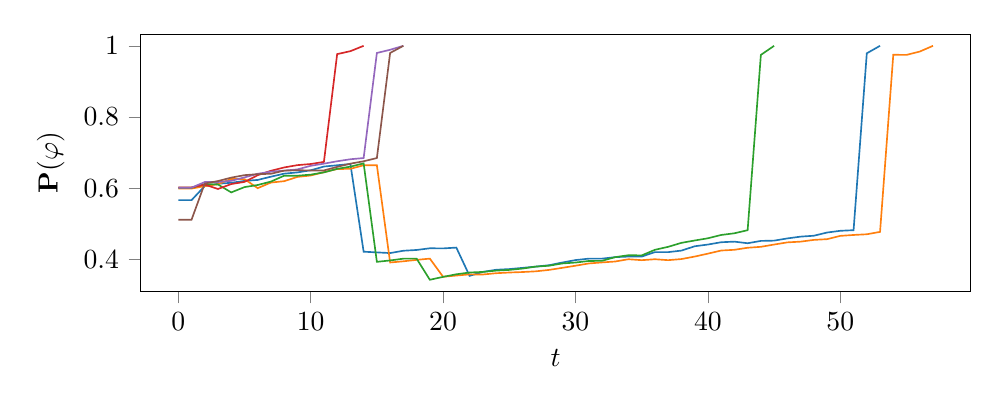
\begin{tikzpicture}

\definecolor{color1}{rgb}{1,0.498039215686275,0.0549019607843137}
\definecolor{color0}{rgb}{0.12156862745098,0.466666666666667,0.705882352941177}
\definecolor{color3}{rgb}{0.83921568627451,0.152941176470588,0.156862745098039}
\definecolor{color2}{rgb}{0.172549019607843,0.627450980392157,0.172549019607843}
\definecolor{color5}{rgb}{0.549019607843137,0.337254901960784,0.294117647058824}
\definecolor{color4}{rgb}{0.580392156862745,0.403921568627451,0.741176470588235}

\begin{axis}[
xlabel={$t$},
ylabel={$\mathbf{P}(\varphi)$},
xmin=-2.85, xmax=59.85,
ymin=0.309747329953731, ymax=1.03286917476414,
width=\figurewidth,
height=\figureheight,
tick align=outside,
tick pos=left,
x grid style={lightgray!92.026143790849673!black},
y grid style={lightgray!92.026143790849673!black}
]
\addplot [semithick, color0, forget plot]
table {%
0 0.566291945691099
1 0.566291945691099
2 0.605882976959095
3 0.612354132971019
4 0.615146535917152
5 0.620313388350838
6 0.623169341037894
7 0.632266923722546
8 0.640795190330476
9 0.64428856744584
10 0.650176429635556
11 0.660779548866506
12 0.664373678411201
13 0.667953572290617
14 0.421487160337076
15 0.419564608493884
16 0.417651962548887
17 0.424169566255033
18 0.426345484650421
19 0.431108756242508
20 0.430751120445197
21 0.433029533909929
22 0.353661706426471
23 0.364637651177082
24 0.370746361215414
25 0.37264879516636
26 0.376096476554164
27 0.379620817426667
28 0.383550124204373
29 0.391056861177142
30 0.39796847687288
31 0.401987604739196
32 0.401987604739196
33 0.406226636436034
34 0.407820359358916
35 0.407820359358916
36 0.420304021230006
37 0.420304021230006
38 0.42456412044507
39 0.436771444246203
40 0.441603593594625
41 0.448081549786945
42 0.449753168781144
43 0.445279132077021
44 0.451811534468228
45 0.452584707531843
46 0.458834058062919
47 0.463837652206807
48 0.466371302770852
49 0.475377310315368
50 0.480216293606419
51 0.481964418471021
52 0.979000567746948
53 1.00000000000003
};
\addplot [semithick, color1, forget plot]
table {%
0 0.598873106893363
1 0.598873106893363
2 0.605763258516315
3 0.611283603809519
4 0.625980214715025
5 0.625459909827864
6 0.600037105448619
7 0.615783090748769
8 0.619663395386156
9 0.631631268283565
10 0.635610395601533
11 0.644933095361082
12 0.653813722584338
13 0.65436717019406
14 0.664376196050784
15 0.664376196050784
16 0.391194641077654
17 0.39449158844791
18 0.398569561919484
19 0.402066086004938
20 0.351017643559466
21 0.354495641612995
22 0.357753716786403
23 0.357448027300466
24 0.361037648081797
25 0.363000703654642
26 0.364351826135898
27 0.366332802416764
28 0.370333602490567
29 0.376096476554164
30 0.382103918728858
31 0.388433862060699
32 0.391350166843864
33 0.393961099841666
34 0.400345432182816
35 0.397687899557991
36 0.400345432182816
37 0.397687899557991
38 0.400830536195599
39 0.407820359358916
40 0.416058418568295
41 0.424766183285142
42 0.426835340818511
43 0.432593309323277
44 0.435217212533577
45 0.441603593594625
46 0.447698345266371
47 0.449753168781144
48 0.454659795944692
49 0.456741221849416
50 0.465971992228634
51 0.468495063144782
52 0.470483407603405
53 0.477188615270852
54 0.974807847155171
55 0.97447871718955
56 0.983895819293738
57 1.00000000000003
};
\addplot [semithick, color2, forget plot]
table {%
0 0.601199049439663
1 0.601199049439663
2 0.611373258769312
3 0.610391266774897
4 0.588067759334584
5 0.602984496882264
6 0.608897306800381
7 0.618585889338314
8 0.635067159607474
9 0.635067159607474
10 0.637973913118502
11 0.644381541950961
12 0.65436717019406
13 0.660484909455385
14 0.669684511424162
15 0.393003778434089
16 0.396899359955564
17 0.40193179843639
18 0.402063552462882
19 0.342616504717841
20 0.350786246779302
21 0.358054890346787
22 0.363000703654642
23 0.364663373600934
24 0.368325353453023
25 0.370333602490567
26 0.374066007307278
27 0.379620817426667
28 0.382103918728858
29 0.388433862060699
30 0.391056861177142
31 0.395396597852448
32 0.395843757502286
33 0.406226636436034
34 0.411622227786086
35 0.411102776012047
36 0.426835340818511
37 0.435217212533577
38 0.44636738575792
39 0.452967252093275
40 0.459226598400379
41 0.468495063144782
42 0.473231351019953
43 0.481964418471021
44 0.97447871718955
45 1.00000000000003
};
\addplot [semithick, color3, forget plot]
table {%
0 0.60221316758681
1 0.60221316758681
2 0.609951541443793
3 0.597706884209307
4 0.611532450112496
5 0.617660129330445
6 0.636414899093264
7 0.648796003646427
8 0.658248408361513
9 0.66472112160367
10 0.667879099243234
11 0.673823637438148
12 0.97666324226307
13 0.984943431279268
14 1.00000000000003
};
\addplot [semithick, color4, forget plot]
table {%
0 0.601395515122941
1 0.601395515122941
2 0.617267794147358
3 0.617267794147358
4 0.620623408292391
5 0.630267741952442
6 0.640464676396021
7 0.646304341196851
8 0.649268206152165
9 0.652756759496805
10 0.66282104615037
11 0.668894859534889
12 0.675589808311553
13 0.681259118631296
14 0.684652063792403
15 0.979868000829901
16 0.988871921656922
17 1.00000000000003
};
\addplot [semithick, color5, forget plot]
table {%
0 0.511047337255817
1 0.511047337255817
2 0.612978700250407
3 0.620063167202848
4 0.629655462002696
5 0.636566259324421
6 0.639381577063717
7 0.640464676396021
8 0.649268206152165
9 0.650371248841046
10 0.649819559965179
11 0.649819559965179
12 0.659844019602223
13 0.668894859534889
14 0.675589808311553
15 0.684652063792403
16 0.979868000829901
17 1.00000000000003
};
\end{axis}

\end{tikzpicture}
	\caption{Same as Fig. \ref{fig:exp1} with the difference that both $O_1$ and $O_2$ contain obstacles.}
	\label{fig:exp2}
\end{figure}